% vim: set tw=78 tabstop=4 shiftwidth=4 aw ai:
\documentclass{beamer}

\usepackage[utf8x]{inputenc}		% diacritice
\usepackage[romanian]{babel}
\usepackage{color}			% highlight
\usepackage{alltt}			% highlight

% highlight; comment this out in case you don't input code source files
%\usepackage{code/highlight}		% highlight

\usepackage{hyperref}			% folosiți \url{http://...}
					% sau \href{http://...}{Nume Link}
\usepackage{verbatim}

% Show contents at every section beginning. Ripped off from manual.
\AtBeginSection[] % Do nothing for \section*
{
    \begin{frame}<beamer>
        \frametitle{Outline}
    \tableofcontents[currentsection]
        \end{frame}
}

\mode<presentation>
{ \usetheme{Berlin} }

% Încărcăm simbolurilor Unicode românești în titlu și primele pagini
\PreloadUnicodePage{200}

\title[Git Repositories]{Gestiunea repository-urilor folosind soluții Git}
\subtitle{Linux and Open Source}
\author[Răzvan Deaconescu]{Răzvan Deaconescu\\
	razvan@rosedu.org}
\date{24 februarie 2011}

\begin{document}

% Slide-urile cu mai multe părți sunt marcate cu textul (cont.)
\setbeamertemplate{frametitle continuation}[from second]

% Arătăm numărul frame-ului
%\setbeamertemplate{footline}[frame number]

\frame{\titlepage}

\frame{\tableofcontents}

% NB: Secțiunile nu sunt marcate vizual, ci doar apar în cuprins
\section{Git}

% Titlul unui frame se specifică fie în acolade, imediat după \begin{frame},
% fie folosind \frametitle
\begin{frame}{Sisteme de versionare a codului}
	\begin{itemize}		% Just like normal LaTeX
		\item Version Control System (VCS), Source Code Management (SCM)
		\item repository, repository URL
        \item working copy/clone
        \item commit, checkout, push, pull, HEAD, branch, merge, tag, trunk
        \item centralizat: Subversion, Perforce
        \item descentralizat: Git, Mercurial, Darcs
	\end{itemize}
\end{frame}

\begin{frame}{Git}
	\begin{itemize}
		\item model descentralizat: fiecare utilizator deține o copie
        \textbf{completă} a repository-ului
		\item ``very fast and scalable''
        \item dezvoltare neliniară și distribuită
        \item facil de creat și gestionat branch-uri
	\end{itemize}
\end{frame}

\begin{frame}{URL-uri Git}
	\begin{itemize}
		\item SSH (autentificare pe bază de parolă sau chei)
          \begin{itemize}
            \item \url{razvan@swarm.cs.pub.ro:git-repos/slides.git}
          \end{itemize}
		\item HTTP(S)
          \begin{itemize}
            \item \url{http://swarm.cs.pub.ro/git/razvan-code.git}
          \end{itemize}
        \item gitdaemon
          \begin{itemize}
            \item \url{git://github.com/vmchecker/vmchecker.git}
          \end{itemize}
	\end{itemize}
\end{frame}

\begin{frame}{Git peste SSH}
	\begin{itemize}
		\item avantaje
          \begin{itemize}
            \item securizat
            \item privat
            \item evitarea parolei (cheie publică)
            \item ușor de configurat
          \end{itemize}
		\item dezavantaje
          \begin{itemize}
            \item problematic de partajat
            \item (în general) necesită un cont Unix
          \end{itemize}
	\end{itemize}
\end{frame}

\begin{frame}{Git peste HTTP}
	\begin{itemize}
		\item avantaje
          \begin{itemize}
            \item universal disponibil (portul 80)
            \item configurare facilă în cadrul unui server web
          \end{itemize}
		\item dezavantaje
          \begin{itemize}
            \item lent
            \item configurare suplimentară pentru push (post-update hook) sau
            autentificare
          \end{itemize}
	\end{itemize}
\end{frame}

\begin{frame}{Protocolul Git}
	\begin{itemize}
		\item avantaje
          \begin{itemize}
            \item rapid
            \item simplu
          \end{itemize}
		\item dezavantaje
          \begin{itemize}
            \item posibilități reduse de configurare a permisiunilor (în
            general read-only)
            \item configurare daemon/serviciu nou
            \item not Internet friendly port (9418)
          \end{itemize}
	\end{itemize}
\end{frame}

\section{Gitolite}

\begin{frame}{Gitolite}
	\begin{itemize}
		\item \url{http://github.com/sitaramc/gitolite}
        \item gestiune centralizată a repository-urilor
        \item acces pe bază de chei publice SSH, fără necesitatea unui cont Unix
          \begin{itemize}
            \item \texttt{command="command"} în \texttt{authorized\_keys}
          \end{itemize}
        \item gestiunea accesului la repository-uri
        \item configurarea tot într-un repository Git (repository-uri, acces,
        chei publice)
	\end{itemize}
\end{frame}

\begin{frame}{Avantaje folosire Gitolite}
	\begin{itemize}
		\item gestiunea repository-urilor se realizează centralizat
		\item crearea repository-urilor se realizează automat la push
        \item controlul accesului
        \item posibilitate de administrare partajată (accesul la repository-ul
        de administrare)
	\end{itemize}
\end{frame}

\section{Gitweb}

\begin{frame}{Gitweb}
	\begin{itemize}
		\item \url{https://git.wiki.kernel.org/index.php/Gitweb}
		\item interfață web pentru vizualizarea repository-urilor
	\end{itemize}
\end{frame}

\begin{frame}{Avantaje folosire Gitweb}
	\begin{itemize}
		\item ușor de configurat și instalat
          \begin{itemize}
            \item \texttt{apt-get install gitweb}
          \end{itemize}
		\item interfață de parcurgere a codului în browser
        \item publicare informații: ownership, URls, description
        \item download snapshots (.zip, .tgz)
	\end{itemize}
\end{frame}

\section{Hosted}

\begin{frame}{GitHub}
  \begin{itemize}
    \item \url{https://github.com/}
    \item ``social coding''
      \begin{itemize}
        \item utilizatorul creează repository-uri
        \item poate invita alți utilizatori
        \item organizații (echipe)
      \end{itemize}
    \item wiki, issues, graphs
    \item HTTP, git, SSH (public key)
    \item comercial -- repository-uri private, colaboratori privați, spațiu
  \end{itemize}
\end{frame}

\begin{frame}{Gitorious}
  \begin{itemize}
    \item \url{http://gitorious.org/}
    \item utilizatori, repository-uri, echipe (similar GitHub)
    \item instalabil pe sistemul local
    \item wiki, code review
    \item HTTP, git, SSH (public key)
    \item suport comercial -- \url{http://gitorious.com/} (nimic concret)
  \end{itemize}
\end{frame}

\section{Scenarii de utilizare}

\begin{frame}{Single user}
	\begin{itemize}
		\item repository local (fără repository URL)
          \begin{itemize}
            \item \texttt{git init . \&\& git add . \&\& git commit -m 'initial commit'}
          \end{itemize}
		\item ``backup'' prin SSH în cazul unui cont Unix
	\end{itemize}
\end{frame}

\begin{frame}{Private party}
	\begin{itemize}
	  \item cont Unix partajat
      \item acces prin SSH (chei publice)
      \item ușor personalizabil (hook-uri)
	\end{itemize}
\end{frame}

\begin{frame}{Private project}
  \begin{enumerate}
    \item Gitolite
      \begin{itemize}
        \item acces SSH pe bază de chei publice
        \item ușor de configurat și administrat
      \end{itemize}
    \item HTTPS
      \begin{itemize}
        \item securizare + autentificare
        \item când se folosește unui cont specializat (username/parolă) (LDAP,
        database etc.)
          \begin{itemize}
            \item Redmine repositories
          \end{itemize}
        \item când este problematic accesul prin chei SSH (pentru Gitolite)
      \end{itemize}
  \end{enumerate}
\end{frame}

\begin{frame}{For the world}
	\begin{enumerate}
		\item Gitolite pentru push (write updates)
          \begin{itemize}
    		\item symlink-uri în \texttt{/var/cache/git} și configurare a
            serverului web (HTTP read-only access)
          \end{itemize}
        \item HTTPS
          \begin{itemize}
            \item HTTP pentru read-only
            \item HTTPS și autentificare pentru push
          \end{itemize}
    \end{enumerate}
    \begin{itemize}
        \item configurare Gitweb
        \item configurare git-daemon (read-only access) (servește din
        /var/cache/git)
	\end{itemize}
\end{frame}

\section{Recomandări}

\begin{frame}{Administrare}
  \begin{itemize}
    \item Gitolite
      \begin{itemize}
        \item gestiunea facilă, centralizată, scalabilă a repository-urilor
      \end{itemize}
    \item GitHub, Gitorious
      \begin{itemize}
        \item outsourcing
      \end{itemize}
  \end{itemize}
\end{frame}

\begin{frame}{All is text}
	\begin{itemize}
		\item scripturi și fișiere de configurare
		\item LaTeX \& LaTeX Beamer
		\item Inkscape -- SVG, Dia -- salvare ca fișier necomprimat (format
		XML)
		\item fișiere de organizare/task-uri (Org-Mode în Emacs)
	\end{itemize}
\end{frame}

\begin{frame}{Versionare și ``diff''-ing}
	\begin{itemize}
		\item versionarea facilă a fișierelor de configurare
		(\texttt{/etc/apache2/})
		\item versionarea temelor submise (studiu de caz UPB)
		\item folosire de tag-uri pentru ani
			\begin{itemize}
				\item se lucrează peste același ``code base''
				\item nu se mai face un director pentru fiecare an
			\end{itemize}
	\end{itemize}
\end{frame}

\begin{frame}{Hook-uri}
	\begin{itemize}
		\item post-receive
		\item trimis e-mail-uri/notificări
		\item creat arhive, compilat prezentări/fișiere LaTeX, publicat
		resurse
			\begin{itemize}
				\item ușor de integrat în wiki-uri
				\item link-ul nu se schimbă, doar conținutul acestuia
                \item problematic de integrat cu Gitolite
			\end{itemize}
	\end{itemize}
\end{frame}

\section{Încheiere}

\begin{frame}{Resurse utile}
	\begin{itemize}
		\item \url{http://git-scm.com/}
        \item \url{http://gitimmersion.com/index.html}
		\item \url{http://progit.org/}
		\item \url{http://github.com/sitaramc/gitolite}
		\item \url{https://git.wiki.kernel.org/index.php/Gitweb}
        \item \url{https://github.com/}
        \item \url{http://gitorious.org/}
	\end{itemize}
\end{frame}

\begin{frame}{Întrebări}
	\begin{columns}
		\begin{column}[l]{0.5\textwidth}
			\begin{itemize}
				\item repository
                \item URL
                \item Git
                \item Gitolite
                \item Gitweb
                \item scenarii
                \item all is text
			\end{itemize}
		\end{column}
		\begin{column}[l]{0.5\textwidth}
			\begin{figure}
				\centering
				\includegraphics[width=0.5\columnwidth]{img/question-mark}
			\end{figure}
		\end{column}
	\end{columns}
\end{frame}

\end{document}
